\begin{figure}[tb]
\centering
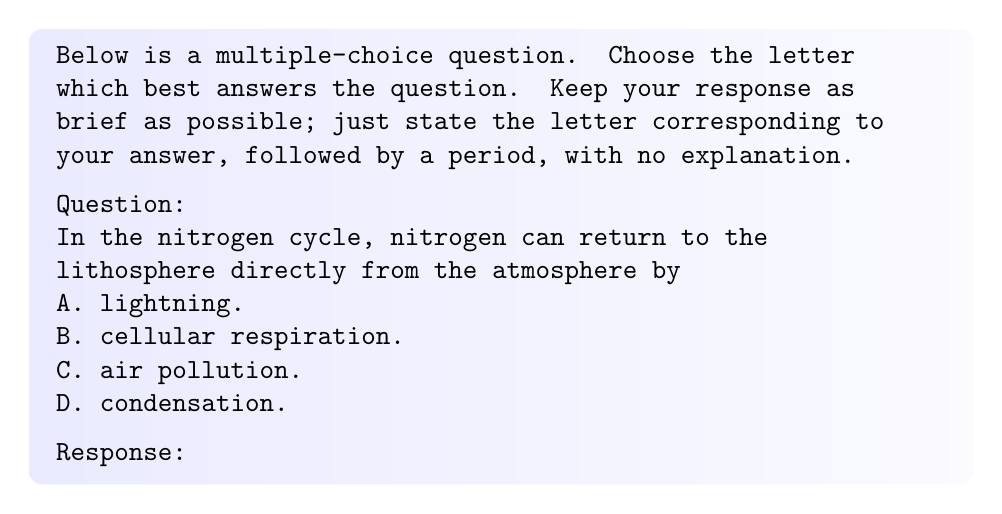
\begin{tikzpicture}
    \draw[white,rounded corners=5pt,path picture={\fill[left color=blue!8, right color=blue!2] (path picture bounding box.south west) rectangle (path picture bounding box.north east);}] (-0.02\linewidth, -2.9) rectangle (0.97\linewidth, 2.9);
    % First prompt
    \node[inner sep=3pt,anchor=west] at (0,0) {
        \fboxrule=0pt
        \parbox{.91\linewidth}{
            {\fontfamily{cmtt}\selectfont
            Below is a multiple-choice question. Choose the letter which best answers the question. Keep your response as brief as possible; just state the letter corresponding to your answer, followed by a period, with no explanation.
            
            \vspace{2mm} % Adds vertical space
            Question:
            
            In the nitrogen cycle, nitrogen can return to the lithosphere directly from the atmosphere by \\
            A. lightning. \\
            B. cellular respiration. \\
            C. air pollution. \\
            D. condensation.
            
            \vspace{2mm} % Adds vertical space
            Response:
            }
        }
    };
\end{tikzpicture}
\caption{A sample question prompt.}
\label{fig:first-prompt}
\end{figure}